% This is based on the LLNCS.DEM the demonstration file of
% the LaTeX macro package from Springer-Verlag
% for Lecture Notes in Computer Science,
% version 2.4 for LaTeX2e as of 16. April 2010
%
% See http://www.springer.com/computer/lncs/lncs+authors?SGWID=0-40209-0-0-0
% for the full guidelines.
%
%------------------------------------------------------------------

\documentclass[twoside,11pt]{article}

\usepackage{jmlr2e}
\usepackage{xcolor}
\usepackage{adjustbox}
\usepackage{booktabs}
\usepackage{siunitx}
\usepackage{listings}
\usepackage{caption}
\usepackage{hyperref}
\usepackage{subcaption}
\usepackage{todonotes}
\usepackage{textcomp}
%\usepackage[variablett]{lmodern}
\usepackage[T1]{fontenc}
% start: uncomment to deactivate inline todos
\makeatletter
\presetkeys%
    {todonotes}%
    {inline}{}%
\makeatother
% end
\usepackage[shortlabels,inline]{enumitem}
\newcommand\hide[1]{}
\newcommand{\numdatasets}{73}

\definecolor{mygreen}{rgb}{0,0.6,0}
\definecolor{mygray}{rgb}{0.5,0.5,0.5}
\definecolor{mymauve}{rgb}{0.58,0,0.82}
\lstset{ %
  backgroundcolor=\color{white},   % choose the background color; you must add \usepackage{color} or \usepackage{xcolor}
  basicstyle=\ttfamily\scriptsize,        % the size of the fonts that are used for the code
  commentstyle=\color{mygreen},    % comment style
  frame=single,	                   % adds a frame around the code
  numbers=left,                    % where to put the line-numbers; possible values are (none, left, right)
  numbersep=5pt,                   % how far the line-numbers are from the code
  numberstyle=\tiny\color{gray},   % the style that is used for the line-numbers
  rulecolor=\color{black},         % if not set, the frame-color may be changed on line-breaks within not-black text (e.g. comments (green here))
  showspaces=false,                % show spaces everywhere adding particular underscores; it overrides 'showstringspaces'
  showstringspaces=false,          % underline spaces within strings only
  showtabs=false,                  % show tabs within strings adding particular underscores
  stringstyle=\color{mymauve},     % string literal style
  breaklines=true,
  breakindent=1em,
  columns=flexible,
  upquote,
}

\ShortHeadings{OpenML-CC18}{Bischl. et al.}
\firstpageno{1}

\begin{document}

\title{OpenML Benchmarking Suites and the OpenML-CC18}
\author{\name Bernd~Bischl \email bernd.bischl@stat.uni-muenchen.de \AND 
	\name Giuseppe~Casalicchio \email giuseppe.casalicchio@stat.uni-muenchen.de \AND
    \name Matthias~Feurer \email feurerm@cs.uni-freiburg.de \AND
    \name Frank~Hutter \email fh@cs.uni-freiburg.de \AND 
    \name Michel~Lang \email lang@statistik.tu-dortmund.de \AND 
    \name Rafael~G.~Mantovani \email rgmantov@icmc.usp.br \AND 
    \name Jan~N.~van~Rijn \email j.n.vanrijn@columbia.edu \AND 
    \name Joaquin~Vanschoren \email j.vanschoren@tue.nl }
 
\editor{To be determined}

\maketitle              % typeset the title of the contribution

% JvR: Important for ArXiv PDF
\hypersetup{pdftitle={OpenML Benchmarking Suites and the OpenML-CC18},pdfauthor={Bernd Bischl, Giuseppe Casalicchio, Matthias Feurer, Frank Hutter, Michel Lang, Rafael G. Mantovani, Jan N. van Rijn, Joaquin Vanschoren}}

%------------------------------------------------------------------
%------------------------------------------------------------------

\begin{abstract}
%Alternative first sentence:
We advocate the use of curated, comprehensive benchmarking suites of machine learning datasets, backed by standardized OpenML-based interfaces and complementary software toolkits written in Python, Java and R.
%
%We demonstrate how to easily execute comprehensive benchmarking studies using standardized OpenML-based benchmarking suites and complementary software toolkits written in Python, Java and R. 
Major distinguishing features of OpenML benchmarking suites are 
\begin{enumerate*}[(a)]
	\item ease of use through standardized data formats, APIs, and existing client libraries; 
    \item machine-readable meta-information regarding the contents of the suite; and
    \item online sharing of results, enabling large scale comparisons.
\end{enumerate*}
As a first such suite, we propose the \textbf{OpenML} \textbf{C}urated \textbf{C}lassification benchmarking suite 20\textbf{18} (OpenML-CC18), a machine learning benchmarking suite of \numdatasets~classification datasets 
carefully curated from the thousands of datasets available on \href{https://www.openml.org}{OpenML.org}.

%\todo{FH: the first part of the abstract only focusses on the actual dataset collection OpenML100, but the second part lists all the distinguishing features of OpenML datasets in general, not those of OpenML100. I think it'd be better to first discuss the great features of OpenML, and then say out of these we curated OpenML100 as a carefully-selected new standard dataset collection.}

%\todo{FH: the longer I think about it the more I am wondering about the title. Reviewers may rightfully ask "so, every time you have a new OpenML-X dataset, you write another paper? Especially for OpenML150, OpenML200, etc, which simply add some datasets?"
%If we don't plan on doing that, having the title focus on OpenML100 might be a strategic mistake, since it would be odd to cite a paper called "OpenML100" for using a future dataset collection OpenML150. But I don't have great alternatives. The best I can think of is: "The OpenML Benchmarking Suite and its Curated Dataset Collection OpenML100".
%But that would be a bit of a deviation from the agreed-upon main message of the paper, so let's discuss. I would also be happy with keeping the initial focus really just on the OpenML100 dataset.}

\begin{keywords}
	machine learning, benchmarking
\end{keywords}
\end{abstract}

%------------------------------------------------------------------
%------------------------------------------------------------------



\section{A Brief History of Benchmarking Suites}
\label{sec:intro}

%\todo{BB: check final nr of datasets in abstract, also section 3}

Proper algorithm benchmarking is a hallmark of machine learning research. It allows us, as a community, to track progress over time, to identify which issues are still challenging, and to learn which algorithms are most appropriate for specific applications. However, we currently lack standardized, easily-accessible benchmarking suites of datasets that are curated to reflect important problem domains, practical to use, and that support a rigorous analysis of performance results.
%Thoroughly setting up experiments, e.g., for a scientific paper, can be difficult and time consuming: it is often not clear which datasets should be included, how to choose training/test splits, and which other algorithms to compare against.
This often results in suboptimal shortcuts in study designs, producing rather small-scale, one-off experiments that should be interpreted with caution \citep{Aha:1992p455}, are hard to reproduce \citep{Pedersen:2008p12980,Hirsh:2008p14360}, and may even lead to contradictory results \citep{Keogh:2003p4930}. Another often criticized aspect is the mindset in benchmarking which focuses too much on competition and dominating the state-of-art, instead of a more fine-grained statistical analysis of large-scale studies, including negative results where popular algorithms fail \citep{sculley2018winner}.
%In order to produce interpretable benchmarks, they should thoroughly explore different conditions, explain how algorithms are affected by different data properties, or at least clearly state under which conditions their results may hold.

The machine learning field has long recognized the importance of dataset repositories. The UCI repository~\citep{Lichman:2013} offers a wide range of datasets, but it does not attempt to make them available through a uniform format or API. The same holds for other repositories, such as LIBSVM~\citep{chang2011libsvm}. \url{mldata.org} is a very popular repository that does provide an API to easily download datasets, and is readily integrated in scikit-learn. However, it is no longer being maintained, and will very likely be merged with our OpenML platform. %\todo{MF: @Joaquin: could you please update this with the current status of OpenML}
KEEL~\citep{KEEL} offers some benchmark data suites, including one for imbalanced classification and one with data sets with missing values. It has a Java toolkit and an R library for convenient access. 

%\todo{MF: maybe reconsider this: - answer to myself: we already have a reference to LibSVM above} The LIBSVM data repository~\citep{chang2011libsvm} focuses on datasets reasonable for SVMs\todo{FH: This might be true, but I have zero evidence for the assumption; please adapt as you see fit. JV: I also have no idea if this is true. Also, why is not having an explicit test set an issue?\\FH: also seeing Matthias' note, why don't we just drop the LibSVM repo here, since we already reference it above?}; it does not provide validation data for all datasets.

%Likewise, 
PMLB~\citep{pmlb} is another collection of datasets, with strong overlap to UCI and tools to import them into Python scripts.
%However, it is unclear why this specific set of datasets was selected.
However, none of the above tools allows to add new datasets or easily share and compare benchmarking results online.\footnote{The latter used to be possible with DELVE (\url{http://www.cs.toronto.edu/~delve/}) and \url{mlcomp.org}, but both services are no longer maintained.}
%that is similarly easy to use as the OpenML100 dataset collection we propose here (at least through Python), but it is not curated as OpenML-CC18, which draws on an order of magnitude more datasets (including those with missing values), only considers datasets large and balanced enough for in-depth analysis, and provides much richer (and extensible) meta-data.
%\todo{FH: I think we agreed that this paragraph on related work should not mention OpenML100 since we haven't introduced it at this point? And it is very odd to mention our new dataset collection for the first time in the middle of related work and start discussing what's great about it. JV: I've taken a shot at rewriting this.}
Other related benchmark collections include UCR~\citep{UCRArchive} for time series data, OpenAI gym~\citep{openai_gym} for reinforcement learning problems, and Mulan~\citep{mulan} for multilabel datasets, with some of the multilabel datasets already being made available on OpenML in \cite{Probst2017}.

All of these existing repositories are 
%\todo{MF: rather is a very subjective word, could we simply drop it?\\FH: fine by me to drop the word.} rather 
curated to some degree, and for many years machine learning researchers have benchmarked their algorithms on a subset of their data sets.
However, most of them do not provide APIs for downloading data in standardized formats into popular machine learning libraries and uploading and comparing the ensuing results. Hence, large scale benchmarks that also build upon previous results of others are still the exception. 
%\todo{FH: is PMLB also an exception? }

\section{OpenML Benchmarking Suites}
We advocate expanding on previous efforts by comprehensive benchmarking suites backed by the open machine learning platform OpenML~\citep{OpenML2013}. Our goal is to substantially facilitate in-depth benchmarking by providing a standard set of datasets covering a wide spectrum of domains and statistical properties, together with rich meta-data and standardized evaluation procedures (i.e., we also provide unified data splits for resampling methods). This eliminates guesswork, makes individual results more comparable, and allows more standardized analysis of all results. In addition, we provide software libraries in several programming languages to easily download these datasets, optionally download prior benchmarking results for reuse and comparison, and to share your results online.  
%This greatly speeds up benchmarking, since it eliminates issues with importing datasets, and drastically reduces the need to run algorithms by other authors. 
%
%[TODO: Shorten this, less focus on OpenML]

%This paper outlines our concept of machine learning benchmarking suites and the complementary software toolkits to easily download these datasets into scientist's existing workflows. We clearly describe a first such benchmarking suite for classification, and demonstrate how to easily include it in existing machine learning software tools.

%%consisting of large but carefully selected benchmarking suites and complementary software toolkits to easily download these datasets into scientist's existing workflows, together with extensive meta-data for deeper analysis of evaluation results, and predefined train-test splits to compare results run by different authors. Researchers can also download and reproduce the benchmarks of other authors and share their own results online. In this paper we clearly describe a first such benchmarking suite for classification, including an overview and analysis of the included datasets, and demonstrate how to easily include it in existing machine learning software tools.

OpenML is an online platform for reproducible, collaborative machine learning experiments and 
can be used to store and share all aspects of machine learning experiments, including data, code, experiment parameters and results.
All our datasets in OpenML are provided in a uniform format, highlight issues such as unique-valued or constant features, include extensive meta-data for deeper analysis of evaluation results, and provide task-specific meta-data, such as target features and predefined train-test splits.

%Researchers can already conveniently explore the OpenML database to find suitable learning tasks for their planned experiments, depending on required data set characteristics (e.g., high-dimensional data sets with few observations and no missing values). 
%However, as the database contains many revised/versioned datasets and data sets of very different quality, a batch selection based solely on the queriable attributes of a dataset is not advisable for many experiments.
%Therefore, researchers should not simply use the available datasets without looking into them and making sure that the datasets they have selected are appropriate for their purpose.
Researchers can conveniently explore the datasets included in OpenML through comprehensive APIs to find suitable learning tasks for their planned experiments, depending on required data set characteristics. These APIs allow, for instance, to find all high-dimensional data sets with few observations and no missing values.

%------------------------------------------------------------------
%------------------------------------------------------------------

\section{The OpenML-CC18 Benchmarking Suite}

On top of OpenML's 
%\todo{MF: not sure if I get the word customizable here\\FH: reworded; please drop the note if this is fine.} 
functionality to provide customized dataset collections through the API, we provide a new standard benchmarking
%\todo{FH: do we call it ``benchmarking suite'' or ``benchmarking suite''? Unify throughout the paper.}
suite of \numdatasets~high-quality classification datasets carefully curated from the many thousands available on OpenML: the OpenML-CC18.

%In order to facilitate this selection process and to provide the machine learning community with a list of high-quality classification datasets, we manually selected 100 datasets among all available datasets on OpenML.
We selected classification datasets for this benchmarking suite to satisfy the following requirements:
%\todo{BB: check the following list, at least at minimal class size}
\begin{enumerate*}[(a)]
  \item the number of observations is between \num{500} and \num{100000} to focus on medium-sized datasets,
  %that are not too small and not too big,
  \item the number of features does not exceed \num{5000}~features to keep the runtime of algorithms low,
  \item the target attribute has at least two classes,
  \item have at least 20 observations per class, and\
  \item the ratio of the minority class and the majority class is above $0.05$ (to eliminate highly imbalanced datasets which require special treatment for both algorithms and evaluation measures).
\end{enumerate*}
%\todo{FH: maybe ``target feature'' is a commonly-used term in some community, but I saw the term for the first time. How about ``target variable''? MF: how about ``attribute``''? I think it is more used than variable.}
We excluded datasets which
\begin{enumerate*}[(a)]
  \item are artificially generated %(not to confuse with simulated) 
  %\todo{MF: there is at least Waveform5000 as an example of an artificial dataset left; we actually removed simulated datasets such as GAMETES, which we treated as artificial in contrast to being simulated)...},
  \item cannot be randomized via a 10-fold cross-validation due to grouped samples or because they are time series or data streams,
  \item are a subset of a larger dataset, %\todo{MF: must it really be on OpenML?} available on OpenML, 
  \item have no source or reference available,
  \item can be perfectly classified by a single attribute or a decision stump,
%\todo{GC: didn't we decide to use linear model and a tree?}
  \item allow a decision tree to achieve 100\% accuracy on a 10-fold cross-validation task,
  \item have more than \num{5000}~features after one-hot-encoding categorical features,
  \item are created by binarization of regression tasks or multiclass classification tasks, or
  \item are sparse data (e.g., text mining data sets).
%which frequently raises technical issues while fitting machine learning models.
\end{enumerate*}
\noindent
A detailed list of the data properties can be found on OpenML\footnote{ \url{https://www.openml.org/s/99}}. 
%Furthermore, we provide a list of datasets with reasons for exclusion in Appendix \ref{app:datasets2}.
%\todo{JvR: I would really opt for using this url, as it is more persistent and future proof}
%\url{https://www.openml.org/search?q=tags.tag=study_14&type=data&table=1}}.

%Figure~\ref{fig:hist} displays the most important properties of the selected datasets in histograms, 

% BB: we remove this to save space, plots are not perfect anyway
% \begin{figure}[ht]
% 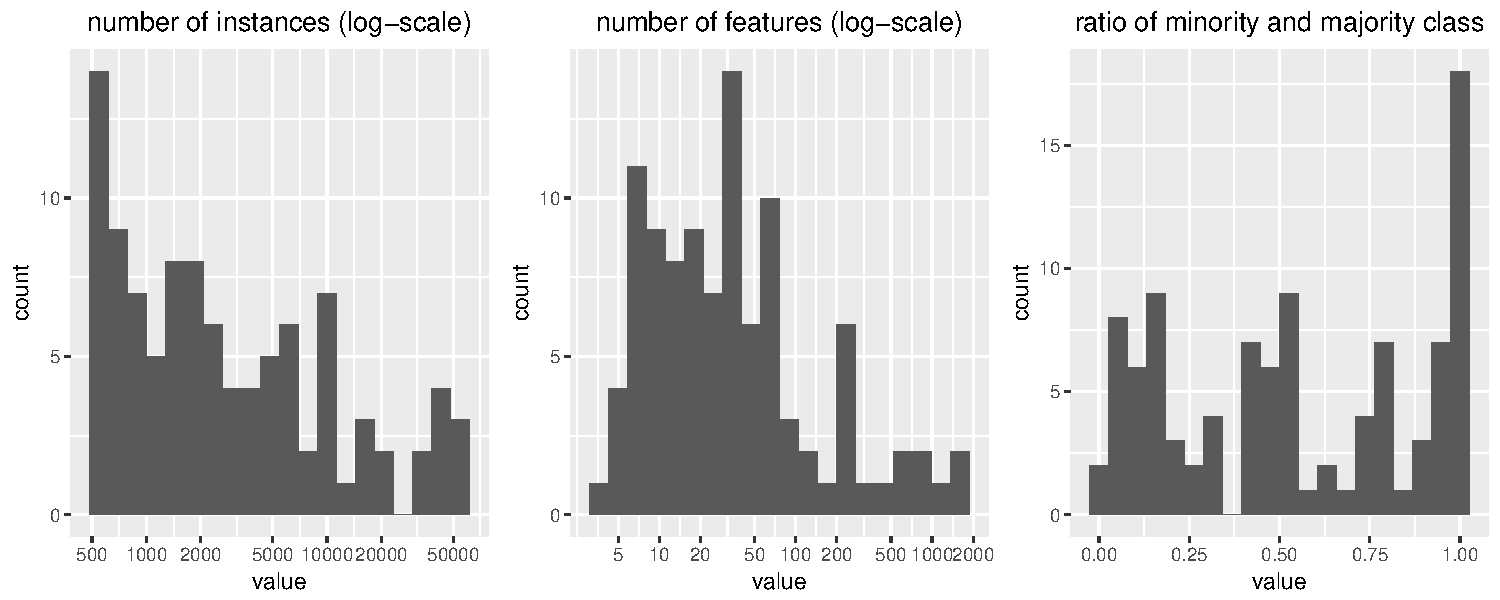
\includegraphics[width = \textwidth]{ds_overview}
% \caption{layout needs to be improved a bit}
% \label{fig:hist}
% \end{figure}

%------------------------------------------------------------------
%------------------------------------------------------------------

\section{How to use the OpenML-CC18}

In this section we demonstrate how our dataset collection can be conveniently imported for benchmarking using our client libraries in Python, Java and R. Figure~\ref{fig:code_examples} provides exemplary code chunks for downloading the datasets and running a basic classifier in all three languages. In these examples, we use the Python library with scikit-learn ~\citep{scikit-learn}, the R package~\citep{Casalicchio2017} with mlr~\citep{Bischl2016}, and the Java library with Weka~\citep{Hall2009}.
%
OpenML has also been integrated in MOA and RapidMiner~\citep{Rijn2015}. 
%\todo{@JvR: this sounds like a shameless self-reference.
%JvR @MF? (please also add name) I don't agree at all. We have chosen to showcase code of several workbenches, which is an arbitrary choose. There is IMO opinion no reason to not list and credit the other packages that we put lots of time and effort in developing.}
%\todo{Is this relevant? Why mention RM and not WEKA/MOA?}

%\todo{update the source code once we have new study getters!}
\begin{figure}[tb]
  \begin{center}
    \begin{subfigure}{\textwidth}
      \lstinputlisting[language=Python]{listings/run_task.py}
      \vspace*{-0.3cm}
      \caption{Python, available on \href{https://github.com/openml/openml-python/}{https://github.com/openml/openml-python/}%\todo{FH: It is suboptimal that performing a run requires the OpenMM API key; this should really only be necessary for uploading the run.}
      }
      \vspace*{0.3cm}
    \end{subfigure} 
    \begin{subfigure}{\textwidth}
      \lstinputlisting[language=Java]{listings/run_task.java}
      \vspace*{-0.3cm}
      \caption{Java, available on Maven Central with artifact id `org.openml.openmlweka'}
      \vspace*{0.3cm}
      \end{subfigure}
    \begin{subfigure}{\textwidth}
      \lstinputlisting[language=R]{listings/run_task.r}
      \vspace*{-0.3cm}
      \caption{R, available on CRAN via package \href{https://CRAN.R-project.org/package=OpenML}{OpenML}} 
      \vspace*{0.3cm}
    \end{subfigure}
    \caption{Running classifiers on a task and (optionally) uploading the results. Uploading requires the user to fill in an API key.\label{fig:code_examples}%\todo{TODO: change name OpenML100 to OpenML-CC18 in all 3 code examples.}
    }
  \end{center}
\vspace{-0.5cm}
\end{figure} % TODO: add negative vspace as the typesetting is too much 
OpenML works with the concept of \emph{tasks} to facilitate comparable and reproducible results.
A task extends a dataset with task-specific information, such as target attributes and evaluation procedures. Datasets and tasks are automatically downloaded at first use and are afterwards cached locally. \emph{Studies} combine a specific set of tasks and can also hold all benchmarking results obtained on them. In the code examples, the OpenML-CC18 tasks are downloaded through the study with the same name. They also show how to access the raw data set (although this is not needed to train a model), fit a simple classifier on the defined data splits, and finally publish runs on the OpenML server. 
%
%\todo{GC: We should keep in mind to remove abalone and anneal online and to replace those data sets. Maybe with data.id 554, 23512, 40536}
Note that the Java implementation automatically uploads results to the server.

%------------------------------------------------------------------
%------------------------------------------------------------------
%  Outlook
\section{Creating new Benchmarking Suites}

The set of datasets on \url{OpenML.org} can easily be extended, and additional OpenML benchmarking suites, e.g., for regression and time-series data, can easily be created by defining sets of datasets according to specific needs. Instructions for creating new benchmarking suites can be found on \url{https://www.openml.org}. We currently envision two routes of extensions:
\begin{enumerate*}[(a)]
\item facilitate the creation and versioning of these benchmarking suites on \url{OpenML.org}; and 
\item adding automatic statistical analysis, visualization and reporting on the online platform.
\end{enumerate*}

%------------------------------------------------------------------
%------------------------------------------------------------------
%  Acknowledgements - founding

\noindent \textbf{Acknowledgements} This work has partly been supported by the European Research Council (ERC) under the European Union's Horizon 2020 research and innovation programme under grant no.\ 716721, through grant \#2015/03986-0 from the S{\~a}o Paulo Research Foundation (FAPESP), as well as Priority Programme Autonomous Learning (SPP 1527, grant HU~1900/3-1) and Collaborative Research Center SFB~876/A3 from the German Research Foundation (DFG).

\clearpage


%------------------------------------------------------------------
%------------------------------------------------------------------
% Bibliography 
\begin{footnotesize}
\bibliography{openml100}
\end{footnotesize}

%------------------------------------------------------------------
%------------------------------------------------------------------

\appendix

\newpage
\begin{table}[h]
% \Huge
\setlength{\tabcolsep}{2pt}
\caption{Datasets included in the OpenML-CC18 benchmarking suite. For each dataset, we show: the OpenML task id, data set id and data set name, the number of classes (cl), features (p) and observations (n), as well as the ratio of the minority and majority class sizes (MinMaj).}
\label{tab:datasets}
\centering

% \begin{adjustbox}{width=\textwidth}
\begin{adjustbox}{center, width=7.75cm, totalheight=12cm}
\begin{tabular}{rrlrrrrr}
\toprule
\textbf{ Data id } & \textbf{Task id} & \textbf{ Name } & \textbf{ cl } & \textbf{ p } & \textbf{ n } & \textbf{MinMaj}\\
\midrule



\midrule
3 & 3 & kr-vs-kp & 2 & 37 & 3196 & 0.91\\
6 & 6 & letter & 26 & 17 & 20000 & 0.90\\
11 & 11 & balance-scale & 3 & 5 & 625 & 0.17\\
12 & 12 & mfeat-factors & 10 & 217 & 2000 & 1.00\\
14 & 14 & mfeat-fourier & 10 & 77 & 2000 & 1.00\\
\addlinespace
15 & 15 & breast-w & 2 & 10 & 699 & 0.53\\
16 & 16 & mfeat-karhunen & 10 & 65 & 2000 & 1.00\\
18 & 18 & mfeat-morphological & 10 & 7 & 2000 & 1.00\\
22 & 22 & mfeat-zernike & 10 & 48 & 2000 & 1.00\\
23 & 23 & cmc & 3 & 10 & 1473 & 0.53\\
\addlinespace
28 & 28 & optdigits & 10 & 65 & 5620 & 0.97\\
29 & 29 & credit-approval & 2 & 16 & 690 & 0.80\\
31 & 31 & credit-g & 2 & 21 & 1000 & 0.43\\
32 & 32 & pendigits & 10 & 17 & 10992 & 0.92\\
37 & 37 & diabetes & 2 & 9 & 768 & 0.54\\
\addlinespace
38 & 3021 & sick & 2 & 30 & 3772 & 0.07\\
44 & 43 & spambase & 2 & 58 & 4601 & 0.65\\
46 & 45 & splice & 3 & 62 & 3190 & 0.46\\
50 & 49 & tic-tac-toe & 2 & 10 & 958 & 0.53\\
54 & 53 & vehicle & 4 & 19 & 846 & 0.91\\
\addlinespace
151 & 219 & electricity & 2 & 9 & 45312 & 0.74\\
182 & 2074 & satimage & 6 & 37 & 6430 & 0.41\\
188 & 2079 & eucalyptus & 5 & 20 & 736 & 0.49\\
300 & 3481 & isolet & 26 & 618 & 7797 & 0.99\\
307 & 3022 & vowel & 11 & 13 & 990 & 1.00\\
\addlinespace
458 & 3549 & analcatdata\_authorship & 4 & 71 & 841 & 0.17\\
469 & 3560 & analcatdata\_dmft & 6 & 5 & 797 & 0.79\\
554 & 3573 & mnist\_784 & 10 & 785 & 70000 & 0.80\\
1049 & 3902 & pc4 & 2 & 38 & 1458 & 0.14\\
1050 & 3903 & pc3 & 2 & 38 & 1563 & 0.11\\
\addlinespace
1053 & 3904 & jm1 & 2 & 22 & 10885 & 0.24\\
1063 & 3913 & kc2 & 2 & 22 & 522 & 0.26\\
1067 & 3917 & kc1 & 2 & 22 & 2109 & 0.18\\
1068 & 3918 & pc1 & 2 & 22 & 1109 & 0.07\\
1461 & 14965 & bank-marketing & 2 & 17 & 45211 & 0.13\\
\addlinespace
1462 & 10093 & banknote-authentication & 2 & 5 & 1372 & 0.80\\
1464 & 10101 & blood-transfusion-service-center & 2 & 5 & 748 & 0.31\\










\bottomrule
\end{tabular}
~~~~~
\begin{tabular}{rrlrrrrr}
\toprule
\textbf{ Data id } & \textbf{ Task id } & \textbf{ Name } &  \textbf{ cl } & \textbf{ p } & \textbf{ n } & \textbf{MinMaj}\\
\midrule 

\midrule
1468 & 9981 & cnae-9 & 9 & 857 & 1080 & 1.00\\
1475 & 9985 & first-order-theorem-proving & 6 & 52 & 6118 & 0.19\\
1478 & 14970 & har & 6 & 562 & 10299 & 0.72\\
1480 & 9971 & ilpd & 2 & 11 & 583 & 0.40\\
1485 & 9976 & madelon & 2 & 501 & 2600 & 1.00\\
\addlinespace
1486 & 9977 & nomao & 2 & 119 & 34465 & 0.40\\
1487 & 9978 & ozone-level-8hr & 2 & 73 & 2534 & 0.07\\
1489 & 9952 & phoneme & 2 & 6 & 5404 & 0.42\\
1494 & 9957 & qsar-biodeg & 2 & 42 & 1055 & 0.51\\
1497 & 9960 & wall-robot-navigation & 4 & 25 & 5456 & 0.15\\
\addlinespace
1501 & 9964 & semeion & 10 & 257 & 1593 & 0.96\\
1510 & 9946 & wdbc & 2 & 31 & 569 & 0.59\\
1590 & 7592 & adult & 2 & 15 & 48842 & 0.31\\
4134 & 9910 & Bioresponse & 2 & 1777 & 3751 & 0.84\\
4534 & 14952 & PhishingWebsites & 2 & 31 & 11055 & 0.80\\
\addlinespace
4538 & 14969 & GesturePhaseSegmentationProcessed & 5 & 33 & 9873 & 0.34\\
6332 & 14954 & cylinder-bands & 2 & 40 & 540 & 0.73\\
23381 & 125920 & dresses-sales & 2 & 13 & 500 & 0.72\\
23517 & 167120 & numerai28.6 & 2 & 22 & 96320 & 0.98\\
40499 & 125922 & texture & 11 & 41 & 5500 & 1.00\\
\addlinespace
40668 & 146195 & connect-4 & 3 & 43 & 67557 & 0.15\\
40670 & 167140 & dna & 3 & 181 & 3186 & 0.46\\
40701 & 167141 & churn & 2 & 21 & 5000 & 0.16\\
40923 & 167121 & Devnagari-Script & 46 & 1025 & 92000 & 1.00\\
40927 & 167124 & CIFAR\_10 & 10 & 3073 & 60000 & 1.00\\
\addlinespace
40966 & 146800 & MiceProtein & 8 & 82 & 1080 & 0.70\\
40975 & 146821 & car & 4 & 7 & 1728 & 0.05\\
40978 & 167125 & Internet-Advertisements & 2 & 1559 & 3279 & 0.16\\
40979 & 146824 & mfeat-pixel & 10 & 241 & 2000 & 1.00\\
40981 & 146818 & Australian & 2 & 15 & 690 & 0.80\\
\addlinespace
40982 & 146817 & steel-plates-fault & 7 & 28 & 1941 & 0.08\\
40983 & 146820 & wilt & 2 & 6 & 4839 & 0.06\\
40984 & 146822 & segment & 7 & 20 & 2310 & 1.00\\
40994 & 146819 & climate-model-simulation-crashes & 2 & 21 & 540 & 0.09\\
40996 & 146825 & Fashion-MNIST & 10 & 785 & 70000 & 1.00\\
\addlinespace
41027 & 167119 & jungle\_chess\_2pcs\_raw\_endgame\_complete & 3 & 7 & 44819 & 0.19\\


 &  &  &  &  &  & \\


\bottomrule
\end{tabular}
\end{adjustbox}
\end{table}

\end{document}

%------------------------------------------------------------------
%------------------------------------------------------------------
